\chapter{Introduction: What Makes Hardware Verification Complex}

Modern hardware designs are extremely complex.
Such a statement has become so hackneyed that it does not draw any attention, but dealing with complex hardware is still a big problem.
A single-core processor and a memory system were enough to run computer programs in the early days.
Computer architecture has become much more complicated, equipped with multicores, various accelerators (\eg{} GPUs, NPUs, etc.), hardware security modules (HSMs), hierarchical memory subsystems, and so on.
Such hardware components form a large, complex hardware circuit often called a system on a chip (SoC).

Concurrency is one of the major challenges in hardware design.
Concurrent execution has been very natural in hardware in terms of maximizing utility of hardware components.
For instance, at a high level, processing units and a memory subsystem run concurrently; \eg{} a processor core may execute other instructions after making a memory request while the memory handles it.
Looking at each component, a processor core may be pipelined, which is very common these days, implying that (computer-architecture) instructions are executed concurrently as well.
The memory subsystem may be composed of several caches and the main memory, and several requests from different cores are handled concurrently in a distributed way throughout the caches and the memory.
Concurrency does not mean complete parallelism; for correctness, some ordering among execution units should be maintained, and managing this constraint is indeed a great challenge.

As hardware has become large with extreme concurrency, hardware verification has become much more challenging as well.
Industry has most commonly used testing and bounded model checking (BMC)~\cite{BMC} for quality assurance of hardware circuits, but these techniques are not sound and may miss subtle bugs.
Due to this shortcoming, both industry and academia have developed so-called \emph{formal-verification} techniques.
At least in hardware verification, there are two mainstream approaches to formally verifying hardware: model checking and theorem proving.

Model checking~\cite{ModelChecking1, ModelChecking2} basically tries to verify a hardware module by exploring all reachable states, checking whether the desired properties hold in those states.
The biggest benefit of model checking is that it is fully automated.
That being said, state-space explosion is a typical problem in model checking; it often requires too much time and (memory) space to explore all reachable states.

Theorem proving, also called deductive verification, provides a mechanism to generate proofs based on a certain logic.
Theorems are proven either manually by a user (called interactive theorem proving), automatically by various solvers (called automated theorem proving), or in a combined way (both interactive and automated).
The biggest benefit of theorem proving is that once a theorem is proven, it can be used repeatedly for bigger proofs.
Theorem provers usually provide rich logics and thus allow a user to state theorems general enough to be reused.
That being said, a theorem prover usually requires a user to understand the target computer system deeply enough to state theorems and proofs in detail.

\subsubsection{Problem statement}

Among various hardware-verification challenges and formal-verification methodologies, this dissertation specifically deals with cache-coherence protocols with the Coq proof assistant~\cite{Coq}, an interactive theorem prover.

Cache-coherence protocols have been regarded as one of the greatest correctness challenges of the hardware world.
As per typical distributed-protocol verification, the main challenge comes while dealing with interleavings among transactions.
In cache-coherence protocols, a request from a processor may require multiple caches to change their local states, and we call a sequence of such state transitions a \emph{transaction}.
Thus it is natural that different cache objects concurrently handle different requests, which makes the transactions \emph{interleaved}.
Interleavings make the verification much more difficult, by significantly increasing the number of states to be explored.

Research on model checking has produced sound techniques to overcome state-space explosion by interleavings.
One of the core techniques is to establish \emph{noninterference} lemmas~\cite{McMillan:1999,McMillan:2001,Chou:2004,flow:Talupur:2008,flow:OLeary:2009,flow:Sethi:2014}, which ensure that concurrent executions of transactions are not spuriously interleaved.
In addition to this resolution, model checkers have supported \emph{parameterization} to verify cache-coherence protocols with unknown numbers of cores~\cite{Zhang:2010,Zhang:2014,Banks:2017}.
In order to cover hierarchical protocols, recent approaches~\cite{Chen:2008,Chen:2010,Opeoluwa:2016,Opeoluwa:2017,Oswald:2020} also employed \emph{modularity} to verify protocols per hierarchy level.

While the same concern exists in theorem proving (by requiring additional proof effort to deal with interlevings), it also has employed similar techniques.
Parameterization is a natural fit for theorem proving, thanks to rich logics, making it possible to prove a cache-coherence protocol with an arbitrary tree shape given as a parameter~\cite{Murali:2015}.
Modularity has been harnessed as well, \eg{} with assume-guarantee reasoning~\cite{McMillan:2016}.

The established style of noninterference reasoning, though, has an inherent weakness: it requires explicit lemma statements per-protocol.
The lemmas are often described explicitly by the user (guided by intuition) or discovered automatically (typically guided by counterexamples).
Another issue is that even though these lemmas are stated and proven, it is hard to be sure if the lemmas are enough to resolve all possible interleavings in the system.

Use of modularity has also imposed significant restrictions in protocol design, in order to obtain clear module boundaries among caches.
A concrete limitation of modular design and verification comes when trying to verify cache-coherence protocols that are not \emph{inclusive}.
Noninclusive caches have been in common industrial use for a decade: AMD Opteron servers are known to use exclusive caches~\cite{Irazoqui:2016}, and Intel Skylake-X processors use noninclusive caches~\cite{intel-non-inclusive,Zhao:2010,Yan:2019}.

We would like to avoid all of these weaknesses via a new approach doing mechanized proof in an expressive logic, stating and proving once-and-for-all a general property and using it multiple times.
Particularly, in proving cache-coherence protocols, we want to formalize \emph{the most-general form of noninterference}, find minimal and abstract conditions \emph{that are not coupled to any specific protocols} but still imply noninterference, state the implication as a theorem, prove it once, and use it repeatedly for various cache-coherence protocols.

The abstract conditions that imply noninterference can be found from the intuitions that protocol designers already have.
In order to describe a case where the protocol deals with two different requests passing through the same cache, for instance, a designer often says ``this cache acts like a \emph{serialization point} so the two transactions can safely \emph{interleave} with each other.''
While the notions of interleaving and serialization are already pervasive, we have found no past work trying to find a minimal set of conditions that ensure transactions are always serialized, formalizing them in a reusable framework.

We go one step further: rather than requiring the user to prove the conditions per-protocol, we establish a framework that guides the user to design protocols that automatically satisfy the conditions, without worrying about possible complex interleavings among different transactions.
The framework does not require the user to write any noninterference properties or to design the protocol in a modular manner.

In this paper, we introduce the \hemiola{} framework, embedded in the Coq proof assistant, which eliminates the burden of designing and proving correct interleavings in cache-coherence protocols.
Specifically, \hemiola{} formalizes a set of message-passing distributed protocols with tree hierarchies and particular topologies of channels between nodes, with associated locks.
\hemiola{} exposes a domain-specific language of protocols, such that any expressible protocol is guaranteed to exhibit ``general'' noninterference, which will be called \emph{serializability} and formalized later in the dissertation.

Furthermore, \hemiola{} provides a novel invariant proof method that only requires consideration of execution histories that do not interleave memory accesses -- so that almost all formal reasoning about concurrency is already done by the framework, not proofs of individual protocols.

To demonstrate usability of our framework, we provide complete correctness proofs for hierarchical cache-coherence protocols, in both inclusive and noninclusive variants, as case studies.
We also demonstrate that the case-study protocols are indeed hardware-synthesizable, by using a compilation/synthesis toolchain in \hemiola{}.

All the code and proofs of the framework and the case studies are available as open source at the following link:
\begin{center}
  \url{https://github.com/..}
\end{center}

\subsubsection{Contributions}

To sum up, the contributions of this dissertation include the following:
\begin{itemize}
\item We discover a minimal set of topology and lock conditions that ensures \emph{serializability}, extracted from usual cache-coherence protocol designs.
  We then identify a domain-specific protocol language, where every protocol defined in this language ensures serializability by construction, backed up with mechanized Coq proof (\autoref{sec-hemiola-dsl}).
  Lastly, we formalize how serializability helps prove correctness (trace refinement), by using the novel notion of \emph{predicate messages} in distributed protocols.
\item Using the protocol language, we provide the complete correctness proofs of three hierarchical cache-coherence protocols: inclusive and noninclusive MSI protocols and a noninclusive MESI protocol (\autoref{sec-case-study}).
  Ours are the first complete mechanized proofs for various hierarchical ``noninclusive'' cache-coherence protocols, and as a bonus they share a large segment of reusable proofs (including with the inclusive variant).
\item We provide a toolchain to compile \hemiola{} protocols to hardware implementations and to synthesize them to run on FPGAs.
  We also evaluate our case-study protocols, in order to demonstrate that they indeed run on hardware with reasonable performance.
\end{itemize}

\subsubsection{Outline}

Before introducing our proposed techniques to verify cache-coherence protocols, we will provide some background in \autoref{sec-background} to understand conventional protocol designs and typical correctness challenges.
After the background chapter, this dissertation is composed of three parts.

The first part presents our underlying theory to reason about cache-coherence protocols.
\autoref{sec-trs} introduces protocol transition systems as underlying state-transition systems to describe behaviors of cache-coherent memory subsystems.
On top of a protocol transition system, we provide the formal definition of serializability in \autoref{sec-sz-def}.
This chapter also demonstrates how serializability helps state and prove invariants of a given system.

The second part introduces \hemiola{}, a framework embedded in Coq to design and verify cache-coherence protocols more structurally, by using the serializability guarantee.
\autoref{sec-hemiola-dsl} first presents the \hemiola{} domain-specific language for easier protocol design.
\autoref{sec-sz-guarantee-hemiola} describes the biggest contribution of the framework, a general once-and-for-all property claiming that any protocol defined with the DSL obtains serializability for free.
We then discuss the first series of related work in \autoref{sec-related-work-i}, focusing on how previous approaches dealt with interleavings among transactions.

The last part provides our case studies to demonstrate practicality of the framework.
We present the designs and complete correctness proofs of hierarchical MSI and MESI protocols on top of \hemiola{} in \autoref{sec-case-study}.
\autoref{sec-comp-syn} presents the protocol compiler, which compiles a protocol described in \hemiola{} to a corresponding hardware implementation and discusses the correctness of the compiler.
We then discuss the other series of related work in \autoref{sec-related-work-ii}, exploring some previous approaches to verifying cache-coherence protocols.

\chapter{Background and Overview}
\label{sec-background}

Before introducing our proposed method to design and prove cache-coherence protocols more structurally, in this chapter we provide some background to understand conventional cache-coherence protocol designs and typical correctness challenges.
We first introduce a very simple cache-coherence protocol to explain the purpose of the protocol, basic design, and a number of nontrivial corner cases that require careful design.
After that, we explore the design space of cache-coherence protocols for better understanding of the case-study protocols that we will provide in \autoref{sec-case-study}.

\section{Cache-Coherence Protocols In a Nutshell}
\label{sec-nutshell}

In this section, we provide a simple yet motivating example to explain the typical challenges.
For simplicity, throughout the section, we will consider a protocol protecting only \emph{a single memory location}.
We will see it is still nontrivial to design and verify a correct protocol.

The overall goal of cache coherence is, as the name suggests, to preserve coherence among multiple candidate values in a memory subsystem.
In other words, if the system is coherent, then it should behave like an atomic memory.
This behavior inclusion is formally defined as \emph{refinement}, which will be introduced in \autoref{sec-semantics}.
The correctness of a cache-coherence protocol is sometimes shown by proving representative invariants, not talking about the relation to the desired spec.
The single-writer/multiple-reader (SWMR) invariant and the data-value invariant~\cite{ccbook:2020} are classic choices; in proving the refinement of a protocol, these invariants (or similar ones) must be proven.

\begin{figure}[t]
  \centering
  \begin{tikzpicture}
    \pic at (0, 0) {skeleton-pcce12={$P(S, v, S_{\tuple{1, 2}})$}{$C_1(S, v)$}{$C_2(S, v)$}};
    \pic at (0, 0) {skeleton-midx-e1};
    \pic at (0, 0) {skeleton-midx-e2};
    \pic at (0, 0) {skeleton-midx-pc1};
    \pic at (0, 0) {skeleton-midx-pc2};
    \node at (3.0, -1) {$\sqsubseteq$};
    \pic at (4.5, -0.7) {spec};
  \end{tikzpicture}
  \caption{A simple MSI directory protocol and its spec}
  \label{fig-motive-1}
\end{figure}

\autoref{fig-motive-1} shows caches and communication channels for a simple directory-based MSI protocol (LHS of $\sqsubseteq$).
Since we deal with only a single memory location, the specification (RHS of $\sqsubseteq$) is a single-value ($v$) container with atomic read and write.
There are three caches ($P$, $C_1$, and $C_2$) in the implementation, and each of them has its own status (M, S, or I) and data ($v$).
The status of a cache represents a permission on its local replica.
In this MSI protocol, an object can read/write the data with the M (``modified'') status, only read with S (``shared''), and cannot read/write with I (``invalid'').
The parent $P$ additionally has a data structure called a \emph{directory} to track the statuses of the children.
For example, a directory might be $S_{\tuple{1, 2}}$, meaning that both $C_1$ and $C_2$ have S status, in some logical snapshot of state.

Objects communicate through ordered channels, shown as $(\rightarrowtail)$ in the figure, where each has a unique index (shown as a natural number in the figure).
$C_1$ and $C_2$ have channels to receive and respond to external requests (from processor cores).
There are three types of channels between a parent and a child: a single channel for parent-to-child messages and two channels for child-to-parent requests and responses, respectively.
It is natural to wonder why two separate channels are required from a child to a parent; we will see the reason very soon.
Note that channels are depicted in a logical way; the actual hardware implementation may use different hardware components (\eg{} finite-capacity FIFOs or buses) that can simulate ordered channels.

\begin{figure}[t]
  \centering
  \begin{tikzpicture}
    \pic at (0, 0) {skeleton-pcce12={$P(S, v, S_{\tuple{1, 2}})$}{$C_1(S, v)$}{$C_2(S, v)$}};
    % C_1 external
    \pic at (0, 0) {skeleton-midx-e1};
    \node[label={[label distance=-6pt,myred]left:{\rdrecmsgsm{a}{rqWr}}},color=myred] at (-1.8, -2.35) {$\bullet$};
    % C_2 external
    \pic at (0, 0) {skeleton-midx-e2};
    \node[label={[label distance=-6pt,myblue]left:{\blrecmsgsm{e}{rqWr}}},color=myblue] at (1.6, -2.35) {$\bullet$};
    % Between P and C_1
    \pic at (0, 0) {skeleton-midx-pc1};
    \node[label={[label distance=-6pt,myred]left:{\rdrecmsgsm{b}{rqM}}},color=myred] at (-1.1, -0.8) {$\bullet$};
    % Between P and C_2
    \pic at (0, 0) {skeleton-midx-pc2};
    \node[label={[label distance=-9pt,myred]below right:{\rdrecmsgsm{d}{rsI}}},color=myred] at (0.9, -0.8) {$\bullet$};
    \node[label={[label distance=-9pt,myred]above right:{\rdrecmsgsm{c}{rqI}}},color=myred] at (1.1, -0.8) {$\bullet$};
    \node[label={[label distance=-9pt,myblue]below left:{\blrecmsgsm{f}{rqM}}},color=myblue] at (0.7, -0.8) {$\bullet$};

    % Curves
    \draw [->,color=myred] (-2.95, -2.05) to[out=90,in=-110] node {\rdcircf{1}} (-2.35, -1.05);
    \draw [->,color=myred] (-2.25, -0.5) to[out=70,in=110,distance=2cm] node {\rdcircf{3}} (1.7, -0.2);
    \draw [->,color=myred] (2.2, -0.7) to[out=-40,in=-40,distance=1.2cm] node {\rdcircf{4}} (2.0, -1.1);
    \draw [->,color=myblue] (0.7, -2.0) to[out=90,in=-45] node {\blcircf{2}} (0.3, -1.4);

  \end{tikzpicture}
  \caption{Rule-execution cases in the simple MSI protocol}
  \label{fig-motive-2}
\end{figure}

\autoref{fig-motive-2} depicts some example state-transition cases depending on statuses of the caches.
All the caches run concurrently, repeatedly executing \emph{rules} that define local state transitions.
A rule may take some messages from input channels, perform a state transition, and put messages in output channels.
A rule may also have a precondition, blocking use of that rule when the precondition does not hold.
$\rdcircf{1}$ shows the case where a child $C_1$ takes an external request (\rdrecmsgsm{a}{rqWr}) to write data, but it does not have M status and thus further requests to the parent (\rdrecmsgsm{b}{rqM}) to get the permission.
At this moment, in many cache-coherence protocol designs, $C_1$ changes its status to a \emph{transient state} SM to record its current status (S) and the next expected status (M).
This transient state also functions as a \emph{lock} not to allow any further external requests for the value.

Due to the concurrent execution of the caches, we might have another rule executed at the same time.
$\blcircf{2}$ is executed concurrently with $\rdcircf{1}$, where $C_2$ also takes an external request (\blrecmsgsm{e}{rqWr}) with the same purpose, thus requests \blrecmsgsm{f}{rqM} to the parent as well.
Since $\rdcircf{1}$ and $\blcircf{2}$ happened at the same time, now the parent $P$ needs to decide which request to deal with.
Suppose that it decided to handle \rdrecmsgsm{b}{rqM} first.

$\rdcircf{3}$ presents the next execution by $P$, taking the input message \rdrecmsgsm{b}{rqM} and making an \emph{invalidation} request (\rdrecmsgsm{c}{rqI}) to the other child $C_2$ to change its status to I.
This invalidation request is required, since when a child has M the others should not be able to read/write the data.
The parent, at this moment, changes its directory status to a transient state (named $S^D$ in some textbooks) to disallow any other requests from the children.
For instance, the parent should not handle \blrecmsgsm{f}{rqM}, since otherwise it will handle two ``\msgsf{rqM}''s simultaneously, which might lead to an incoherent state -- two M statuses in the caches.

Lastly, $\rdcircf{4}$ shows the case that $C_2$ handles the invalidation request (\rdrecmsgsm{c}{rqI}).
A number of corner cases should be handled carefully:
\begin{itemize}[leftmargin=*]
\item Since $C_2$ requested \blrecmsgsm{f}{rqM}, it has a transient state SM when \rdrecmsgsm{c}{rqI} arrives. It should still be able to handle this invalidation request even in the transient state (while not allowing any external requests). In this case $C_2$ accepts \rdrecmsgsm{c}{rqI} and changes its transient state to IM. We see that transient states should be fine-grained enough to distinguish which requests to handle.
\item Due to the existence of \blrecmsgsm{f}{rqM}, if we had a single channel from a child to a parent, a deadlock would occur. $P$ cannot take \blrecmsgsm{f}{rqM} since it has been locked (in a transient state) after making an invalidation request. It cannot take \rdrecmsgsm{d}{rsI} as well since the response is not the first one of the ordered channel. This case shows the necessity of having multiple channels between a child and a parent.
\end{itemize}

A so-called three-channel system has been widely used and regarded as a good choice to make the design correct and live~\cite{Murali:2015,thesis:Murali:2016}.
While there are other possible correct topology and network settings, the cases shown in \autoref{fig-motive-2} at least demonstrate that it is nontrivial to construct one of them.

\begin{figure}[t]
  \centering
  \begin{tikzpicture}
    \pic at (0, 0) {skeleton-pcce12={$P(S, v, S_{\tuple{1, 2}})$}{$C_1(S, v)$}{$C_2(S, v)$}};
    % C_1 external
    \pic at (0, 0) {skeleton-midx-e1};
    \node[label={[label distance=-6pt,myred]right:{\rdrecmsgsm{i}{rsWr}}},color=myred] at (-1.6, -2.35) {$\bullet$};
    % C_2 external
    \pic at (0, 0) {skeleton-midx-e2};
    % Between P and C_1
    \pic at (0, 0) {skeleton-midx-pc1};
    \node[label={[label distance=-12pt,myred]below right:{\rdrecmsgsm{g}{rsM}}},color=myred] at (-0.9, -1.0) {$\bullet$};
    \node[color=myblue] at (-0.5, -0.6) {$\bullet$};
    \node at (-1.5, -0.3) {\blrecmsgsm{h}{rqI}};
    \draw [densely dashed,color=myblue,line width=0.3pt] (-0.5, -0.6) to[out=170,in=-10] (-1.1, -0.3);

    \node[color=myblue] at (-0.8, -0.7) {$\bullet$};
    \node at (-2.5, -0.5) {\blrecmsgsm{j}{rsI}};
    \draw [densely dashed,color=myblue,line width=0.3pt] (-0.8, -0.7) to[out=190,in=-10] (-2.05, -0.5);

    % Between P and C_2
    \pic at (0, 0) {skeleton-midx-pc2};
    \node[label={[label distance=-9pt,myred]above right:{\rdrecmsgsm{d}{rsI}}},color=myred] at (0.9, -0.8) {$\bullet$};
    \node[color=myblue] at (0.7, -0.8) {$\bullet$};
    \node at (2.0, 0.2) {\blrecmsgsm{f}{rqM}};
    \draw [densely dashed,color=myblue,line width=0.3pt] (0.7, -0.8) to[out=70,in=210] (1.5, 0.1);

    % Curves
    \draw [->,color=myred] (1.05, -0.5) to[out=180,in=60] node {\rdcircf{5}} (-0.6, -1.1);
    \draw [->,color=myred] (-0.6, -1.5) to[out=-90,in=80] node {\rdcircf{7}} (-0.8, -2.2);
    \draw [->,color=myblue] (2.0, 0.4) to[out=130,in=80,distance=1.5cm] node {\blcircf{6}} (-1.5, -0.1);
    \draw [->,color=myblue] (-1.5, -0.5) to[out=245,in=-115,distance=0.9cm] node {\blcircf{8}} (-2.5, -0.8);
    \draw [->,color=myblue] (-2.5, -0.3) to[out=90,in=-100] (-2.0, 0.7);
    \node[color=myblue] at (-2.0, 1.1) {$\vdots$};

  \end{tikzpicture}
  \caption{Rule-execution cases, continued}
  \label{fig-motive-3}
\end{figure}

\autoref{fig-motive-3} presents some additional rule-execution cases right after $\rdcircf{4}$ in \autoref{fig-motive-2}.
After $\rdcircf{4}$ responds with \rdrecmsgsm{d}{rsI}, now $P$ can take it to respond back to $C_1$.
$\rdcircf{5}$ presents this step, taking \rdrecmsgsm{d}{rsI} and responding back to $C_1$ with \rdrecmsgsm{g}{rsM}.
At this moment $P$ changes its status to $P(I, \cdot, M_{(1)})$ (from the transient state $S^D$) to record that it no longer has the coherent value and just granted $C_1$ the M status.
Since the transient state also functions like a lock, this status change can be also regarded as a lock release, so that $P$ can handle some other requests.

$\blcircf{6}$ is the next transition step by $P$ to accept a new request.
\blrecmsgsm{f}{rqM} has been waiting for the transient state of $P$ to be released, and $\blcircf{6}$ finally takes it and sends an invalidation request to $C_1$.

Looking at the message channel $5$, the one for parent-to-child messages (from $P$ to $C_1$), there are two messages, \rdrecmsgsm{g}{rsM} and \blrecmsgsm{h}{rqI}, residing in the channel.
A single parent-to-child channel affects the correctness of the protocol in this case.
If we had two separated downward channels, one for requests and the other for responses, $C_1$ could handle \blrecmsgsm{h}{rqI} first, change its status to I, handle \rdrecmsgsm{g}{rsM} later, and change its status to M again.
Since it sent the invalidation response to the parent, eventually $C_2$ will also get the M status, which leads to an incoherent state.
Therefore, it is crucial to have a single parent-to-child channel so that \rdrecmsgsm{g}{rsM} \emph{blocks} \blrecmsgsm{h}{rqI} to be handled first.
After $C_1$ takes \rdrecmsgsm{g}{rsM} and responds back to the processor core with \rdrecmsgsm{i}{rsWr}, presented as $\rdcircf{7}$, it can subsequently take the invalidation request \blrecmsgsm{h}{rqI} and responds with \blrecmsgsm{j}{rsI}, as shown in $\blcircf{8}$.

As examined in \autoref{fig-motive-2} and \autoref{fig-motive-3}, in a cache-coherence protocol, transient states and network channels play a crucial role in making \emph{interleavings} correct.
Regarding the sequence of rule executions (in red) $[\rdcircf{1}; \rdcircf{3}; \rdcircf{4}]$ as an execution flow in \autoref{fig-motive-2} -- we will call it a \emph{transaction} in later sections -- to handle the original external request \rdrecmsgsm{a}{rqWr}, we see that no further executions could happen after $\blcircf{2}$, which is for the other request \blrecmsgsm{e}{rqWr}.
As explained above case-by-case, proper transient states and network channels block \blrecmsgsm{f}{rqM} from further processing.
Similarly, in \autoref{fig-motive-3}, the execution flow $[\rdcircf{5}; \rdcircf{3}]$ was not spuriously affected by $\blcircf{6}$ or $\blcircf{8}$, thanks to the correct channel setting.

\revised{Throughout the dissertation, we will use this example to convey various intuitions in formal definitions and proofs, referred to as the ``interleaving example.''}

\section{Overview: the \hemiola{} Framework and Its Formal Guarantee}
\label{sec-overview}

In the previous section, we confirmed that proper locking (by transient states) and topology are crucial for designing a correct cache-coherence protocol.
If such ingredients are that essential, can we craft a domain-specific language where only conformant protocols are expressible?
That is exactly what the \hemiola{} framework provides: it provides \emph{rule templates}, explained in \autoref{sec-rule-templates} in more detail, that employ proven-safe topologies and network structures and automatically set associated locks, so designers can design protocols without worrying about corner cases due to interleavings.

Before diving into the details of the theory, in this section, we provide the brief overview of the \hemiola{} framework by redefining the example protocol shown in \autoref{sec-nutshell} using rule templates.
Specifically, we will show the use of transient states discussed in \autoref{sec-nutshell} directly in conventional description and compare them with the alternative locking mechanism suggested in \hemiola{}.
After the comparison, we will provide high-level intuitions about the formal meaning of safe interleavings and how the rule templates ensure this property.

\subsubsection{The \hemiola{} rule templates}

\newcommand{\cann}[1]{{\color{mygreen}#1}}
\newcommand{\ccompo}[1]{{\color{myred}#1}}
\newcommand{\ccompt}[1]{{\color{myblue}#1}}
\newcommand{\ccomph}[1]{{\color{mygray}#1}}

\begin{figure}[h]
  \centering\footnotesize\tt\frenchspacing
  \renewcommand{\arraystretch}{1.0}
  \begin{tabular}{|c|l|l|}
    \hline
    & {\sf\it Conventional description} & {\sf\it In Hemiola}\\
    \hline
    (1) & \cann{rule} := & \cann{rule}.rquu\\
    & \ccompo{msgIn} = extToC1.first; & :\cann{from} ext\\
    & extToC1.deq(); & :\cann{me} C1\\
    & \cann{assert} (\ccompo{msgIn}.id == rqWr); & :\cann{accepts} rqWr\\[7pt]
    (2) & \cann{assert} (!\ccomph{mshr}.\underline{in\_transition}); & :\cann{requires}\\
    & \cann{assert} (\ccompt{line}.status $\leq$ msiS); & \ (fun \ccompt{line} \ccompo{msgIn} => \ccompt{line}\#[status] $\leq$ msiS)\\[7pt]
    (3) & \ccomph{mshr}.\underline{in\_transition} <= \underline{msiSM}; & :\cann{transition}\\
    & c1ToPRq.enq(\{id: rqM, val: 0\}); & \ (fun \ccompt{line} \ccompo{msgIn} => <| rqM, 0 |>).\\
    & \cann{endrule} & \\
    \hline
  \end{tabular}
  \caption{A child requesting M to its parent}
  \label{fig-overview-1}
\end{figure}

\autoref{fig-overview-1} presents a conventional rule description (in pseudocode) used to request the M status to a parent on the left side of the figure.
This rule definition matches the rules $\rdcircf{1}$ and $\blcircf{2}$ in the interleaving example shown in \autoref{fig-motive-2}.
This figure also presents a corresponding rule in \hemiola{} using one of the rule templates.
There are largely three benefits of using the \hemiola{} rule templates; we explain them by matching the number annotations in the figure.
\begin{enumerate}[(1)]
\item Input/output patterns: in conventional description, a user has to find and designate a FIFO module to dequeue an input message and to check the purpose of the message by looking at its message ID.
  In \hemiola{}, each rule template is restricted in terms of input/output patterns; for instance, the \slstinline{rquu} rule template (where \slstinline{rquu} stands for request-up-up) always takes an input request from one of its children (\slstinline{:from} the \slstinline{ext}ernal world in this case) and generates an output request to the parent of \slstinline{:me C1}.
  We can also annotate that this rule only \slstinline{:accepts} an input message with an ID \slstinline{rqWr}.
\item In-transition checks: conventional description uses a miss status holding register (\ccomph{\slstinline{mshr}}) to record whether a line is \slstinline{in_transition} or not.
  \hemiola{} employs an abstract locking mechanism, and each rule template automatically sets/releases the locks.
  Hence, a user does not need to describe any in-transition checks or transient states manually, which is one of the major headaches in designing a protocol.
  More specifically, \hemiola{} provides two kinds of locks: \emph{an uplock and a downlock}.
  The \slstinline{rquu} rule template automatically sets an uplock, since it makes an upward request (to the parent).
  The uplock is released when handling the corresponding response from the parent.
  We will see some other use cases of the locks in the other rule templates.
\item Use of transient states: in conventional description, a user should manually update \ccomph{\slstinline{mshr}} to set a proper transient state and find a FIFO to enqueue an output message.
  Neither is required in \hemiola{}; in this \slstinline{rquu} rule template we just need to construct an output message.
  All the rule templates assume the three-channel system introduced in \autoref{sec-nutshell}; \eg{} the \slstinline{rquu} rule template enqueues an output message to the upward-request channel.
\end{enumerate}

\begin{figure}[h]
  \centering\footnotesize\tt\frenchspacing
  \renewcommand{\arraystretch}{1.0}
  \begin{tabular}{|c|l|l|}
    \hline
    & {\sf\it Conventional description} & {\sf\it In Hemiola}\\
    \hline
    (1) & \cann{rule} := & \cann{rule}.rqud\\
    & \ccompo{msgIn} = c1ToPRq.first; & :\cann{from} C1\\
    & c1ToPRq.deq(); & :\cann{me} P\\
    & \cann{assert} (\ccompo{msgIn}.id == rqM); & :\cann{accepts} rqM\\[7pt]
    (2) & \cann{assert} (!\ccomph{mshr}.\underline{in\_transition}); & :\cann{requires}\\
    & \cann{assert} (\ccompt{line}.dir.st == msiS); & \ (fun \ccompt{line} \ccompo{msgIn} => \ccompt{line}\#[dir].st == msiS)\\[7pt]
    (3) & \ccomph{mshr}.\underline{in\_transition} <= \underline{msiSD}; & :\cann{transition}\\
    & pToC2.enq(\{id: rqI, val: 0\}); & \ (fun \ccompt{line} \ccompo{msgIn} => (C2, <| rqI, 0 |>).\\
    & \cann{endrule} & \\
    \hline
  \end{tabular}
  \caption{A parent requesting invalidation to the other child sharer}
  \label{fig-overview-2}
\end{figure}

\autoref{fig-overview-2} shows another rule pattern to make a further request, used in the parent object to send an invalidation request to the other sharer.
This rule matches the rules $\rdcircf{3}$ and $\blcircf{6}$ in the interleaving example shown in \autoref{fig-motive-2} and \autoref{fig-motive-3}, respectively.
We have the same three benefits in the suggested rule template on the right side of the figure: to use correct input/output channels, no in-transition checks, and no need to consider transient states.
The only difference from the \slstinline{rquu} template is that this one generates further requests to children, not to the parent.
(\slstinline{rqud} here stands for request-up-down.)
It automatically sets a downlock, since it makes downward requests to children.
Likewise, the downlock is released when handling the corresponding responses from the children.

\begin{figure}[h]
  \centering\footnotesize\tt\frenchspacing
  \renewcommand{\arraystretch}{1.0}
  \begin{tabular}{|c|l|l|}
    \hline
    & {\sf\it Conventional description} & {\sf\it In Hemiola}\\
    \hline
    (1) & \cann{rule} := & \cann{rule}.immu\\
    & \ccompo{msgIn} = pToC2.first; & :\cann{me} C2\\
    & pToC2.deq(); & :\cann{accepts} rqI\\
    & \cann{assert} (\ccompo{msgIn}.id == rqI); & \\[7pt]
    (2) & \cann{assert} (\ccomph{mshr}.\underline{in\_transition} & :\cann{requires}\\
    & \ \ \ \ \ \ \ \ == msiSM); & \ (fun \ccompt{line} \_ \_ => \ccompt{line}\#[status] == msiS)\\[7pt]
    (3) & \ccomph{mshr}.\underline{in\_transition} <= \underline{msiIM}; & :\cann{transition}\\
    & \ccompt{line}.status <= msiI; & \ (fun \ccompt{line} \ccompo{msgIn} =>\\
    & c2ToPRs.enq(\{id: rsI, val: 0\}); & \ \ (\ccompt{line} +\#[status $\leftarrow$ msiI], <| rsI, 0 |>).\\
    & \cann{endrule} & \\
    \hline
  \end{tabular}
  \caption{A child responding to invalidation immediately even in transition}
  \label{fig-overview-3}
\end{figure}

The next pattern, shown in \autoref{fig-overview-3}, is used to respond immediately to a request from a parent.
The rules $\rdcircf{4}$ and $\blcircf{8}$ in the interleaving example use this pattern to handle an invalidation request.
As already discussed in \autoref{sec-nutshell}, the child object should be able to handle this invalidation request from its parent even though it is in transition.
In conventional description, it is required to change the transient state properly (from \slstinline{msiSM} to \slstinline{msiIM} in this example).
In \hemiola{}, as seen in the figure, it is not required to manage such transient states; a user can just use the \slstinline{immu} rule template (where \slstinline{immu} stands for immediate-up).
The locking mechanism using an uplock and a downlock is still enough to implement this case properly by priortizing downward requests to the uplock.

\begin{figure}[h]
  \centering\footnotesize\tt\frenchspacing
  \renewcommand{\arraystretch}{1.0}
  \begin{tabular}{|c|l|l|}
    \hline
    & {\sf\it Conventional description} & {\sf\it In Hemiola}\\
    \hline
    (1) & \cann{rule} := & \cann{rule}.rsud\\
    & \ccompo{msgIn} = c2ToPRs.first; & :\cann{accepts} rsI\\
    & c2ToPRs.deq(); & \\
    & \cann{assert} (\ccompo{msgIn}.id == rsI); & \\[7pt]
    (2) & \cann{assert} (\ccomph{mshr}.\underline{in\_transition}); & :\cann{holding} rqM\\
    & \cann{assert} (\ccomph{mshr}.rq.id == rqM) & :\cann{requires} (fun \_ \_ \_ => True)\\[7pt]
    (3) & \ccomph{mshr}.\underline{in\_transition} <= None; & :\cann{transition}\\
    & \ccompt{line}.dir.st <= msiM; & \ (fun \ccompt{line} \ccompo{msgIn} rq rsbTo =>\\
    & \ccompt{line}.dir.excl <= \ccomph{mshr}.rsbTo; & \ \ (\ccompt{line} +\#[status $\leftarrow$ msiI]\\
    & \ccompt{line}.status <= msiI; & \ \ \ \ \ \ \ \ +\#[dir $\leftarrow$ setDirM rsbTo],\\
    & pToC1.enq(\{id: rsM, val: 0\}); & \ \ \ <| rsM, 0 |>).\\
    & \cann{endrule} & \\
    \hline
  \end{tabular}
  \caption{A parent responding back to the child requestor to grant M}
  \label{fig-overview-4}
\end{figure}

In a usual cache-coherence protocol, when a cache object gets a response message from another object, it must have previously sent a corresponding request to that object.
\autoref{fig-overview-4} describes this case, where a parent cache object handles an invalidation response from a child, like the rule $\rdcircf{5}$ in the interleaving example.
In conventional description, we need to check that the line is currently \slstinline{in_transition} and the original request held in the MSHR matches the input response.
It is also required to release the MSHR slot by setting \slstinline{in_transition} to none.
As expected, in \hemiola{} we do not need to manage transient states at all; the \slstinline{rsud} rule template (standing for response-up-down) just requires additional annotation \slstinline{:holding rqM} to declare that the rule handles a response message where the ID of the original request message is \slstinline{rqM}.
This rule template automatically releases the downlock previously acquired when sending a downward invalidation request.

\begin{figure}[h]
  \centering\footnotesize\tt\frenchspacing
  \renewcommand{\arraystretch}{1.0}
  \begin{tabular}{|c|l|l|}
    \hline
    & {\sf\it Conventional description} & {\sf\it In Hemiola}\\
    \hline
    (1) & \cann{rule} := & \cann{rule}.rsdd\\
    & \ccompo{msgIn} = pToC1.first; & :\cann{accepts} rsM\\
    & pToC1.deq(); & \\
    & \cann{assert} (\ccompo{msgIn}.id == rsM); & \\[7pt]
    (2) & \cann{assert} (\ccomph{mshr}.\underline{in\_transition}); & :\cann{holding} rqWr\\
    & \cann{assert} (\ccomph{mshr}.rq.id == rqWr); & :\cann{requires} (fun \_ \_ \_ => True)\\[7pt]
    (3) & \ccomph{mshr}.\underline{in\_transition} <= None; & :\cann{transition}\\
    & \ccompt{line}.status <= msiM; & \ (fun \ccompt{line} \ccompo{msgIn} rq rsbTo =>\\
    & \ccompt{line}.value <= \ccomph{mshr}.rq.value; & \ \ (\ccompt{line} +\#[status $\leftarrow$ msiM]\\
    & c1ToExt.enq(\{id: rsWr, val: 0\}); & \ \ \ \ \ \ \ \ +\#[value $\leftarrow$ rq.(msg\_value)],\\
    & \cann{endrule} & \ \ \ <| rsWr, 0 |>). \\
    \hline
  \end{tabular}
  \caption{A child responding to the write request}
  \label{fig-overview-5}
\end{figure}

Lastly, \autoref{fig-overview-5} deals with the case where a child finally gets a response from its parent to update its status to M, like the rule $\rdcircf{7}$ in the interleaving example.
The \slstinline{rsdd} rule template (standing for response-down-down) is very similar to the \slstinline{rsud} template but has a difference that it automaticlly releases the uplock that was previously acquired when sending the \slstinline{rqM} request.

We will explore much more details of the locking mechanism and the rule templates provided by \hemiola{} in \autoref{sec-hemiola-dsl}.

\subsubsection{The serializability guarantee by \hemiola{}}

We have emphasized that it is easier to describe cache-coherence protocols with the \hemiola{} rule templates, but it does not mean a lot if the rule templates are just the alternative representation of transient states.
The biggest contribution of the \hemiola{} framework is that using the rule templates (implicitly with the locking mechanism) already implies safe interleavings among transactions.

\hemiola{} provides the formal definition of serializability as a criterion for safe interleavings.
Informally, it claims that for any legal history of a system we can always find a sequential history that reaches the same resulting state, where each transaction is performed atomically (without any interleavings) in it.

\begin{figure}[h]
  \centering
  \renewcommand{\arraystretch}{1.2}
  \setlength\tabcolsep{2.5pt}
  \begin{tabular}{|ccc|}
    \hline
    \multicolumn{1}{|l}{
      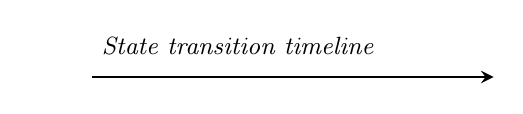
\begin{tikzpicture}
        \node at (0, 0) {};
        \node[anchor=west] at (0.7, 0.4) {{\small\it State transition timeline}};
        \draw [>=stealth,->,line width=1pt] (0.7, 0) to (5.8, 0);
    \end{tikzpicture}} & &
    \multicolumn{1}{l|}{
      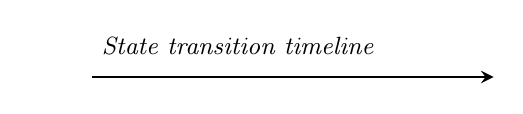
\begin{tikzpicture}
        \node at (0, 0) {};
        \node[anchor=west] at (0.7, 0.4) {{\small\it State transition timeline}};
        \draw [>=stealth,->,line width=1pt] (0.7, 0) to (5.8, 0);
    \end{tikzpicture}}\\
    \begin{tabular}{c|ccccccccc}
      \hline
      $C_1$ & & \rdcircf{1} & & & & & & \rdcircf{7} & \blcircf{8} \\
      \hline
      $P$ & & & & \rdcircf{3} & & \rdcircf{5} & \blcircf{6} & & \\
      \hline
      $C_2$ & & & \blcircf{2} & & \rdcircf{4} & & & & \\
      \hline
    \end{tabular} & $\Rightarrow$ &
    \begin{tabular}{c|ccccccccc}
      \hline
      $C_1$ & & \rdcircf{1} & & & & \rdcircf{7} & & & \blcircf{8} \\
      \hline
      $P$ & & & \rdcircf{3} & & \rdcircf{5} & & & \blcircf{6} & \\
      \hline
      $C_2$ & & & & \rdcircf{4} & & & \blcircf{2} & & \\
      \hline
    \end{tabular}\\
    {\small An original history $h$} & & {\small A sequential history $h_{\textrm{seq}}$}\\
    \hline
  \end{tabular}
  \caption{An example of a serializable history}
  \label{fig-sz-ex}
\end{figure}

\autoref{fig-sz-ex} presents a history brought from the example in \autoref{sec-nutshell}, where two histories (in {\color{myred} red} and {\color{myblue} blue}) are interleaved to form a history $h$.
We can find a corresponding sequential history $h_{\textrm{seq}}$, formed by concatenating two transactions in {\color{myred} red} and {\color{myblue} blue}.
Following the rule executions in $h_{\textrm{seq}}$, we see that it indeed reaches the same state as the original history $h$ does.
We will introduce all the required formalization to define serializability in \autoref{sec-sz-def}.

The biggest contribution of the \hemiola{} framework is that the use of the rule templates implies serializability.
\autoref{fig-sz-ex} just presents a specific history and its corresponding sequential history.
\hemiola{} provides a theorem that we can find a sequential history for any legal history in any protocol designed with the rule templates.
In other words, the theorem says that good request/response patterns with proper locking mechanisms are enough to prove serializability.

How does this nontrivial theorem hold?
The highest-level intuition behind this theorem is the \emph{mutual exclusions} by uplocks and downlocks.
For instance, when an object is uplocked, it cannot generate any further upward requests from it, indicating that only a single transaction can (upwardly) pass through this object by acquiring an uplock.
Likewise, when an object is downlocked, it cannot generate any further downward requests, meaning that a single transaction can (downwardly) pass through this object by acquiring a downlock.

Mutual exclusion by a lock is one typical way to make an execution of a transaction (thread) atomic.
By repeatedly applying the atomicity guarantee by each lock, we can derive a sequential history from a given interleaved one.
Note again that the state transitions by a transaction (other than locking) are irrelevant to the locking mechanism, implying that the serializability proof indeed does not require any specific conditions on a protocol.

All the required proof techniques to reason about these mutual exclusions and the actual serializability proof will be introduced in \autoref{sec-sz-guarantee-hemiola}.
We will also present our suggested methodology to exploit serializability for the verification of cache-coherence protocols in \autoref{sec-pred-msg}.

\section{Design Space of Cache-Coherence Protocols}
\label{sec-design-space}

In \autoref{sec-nutshell} and \autoref{sec-overview}, we examined a very specific protocol design.
There are different ways to design a cache-coherence protocol, and each design decision affects performance and correctness of the protocol.
In this section, we explore the major design space of conventional cache-coherence protocols.

\subsubsection{Snooping vs. Directory}

A typical classification of a cache-coherence protocol is whether the protocol employs a designated data structure to keep track of the statuses of child caches.
There are two representative classes: \emph{snooping} and \emph{directory} protocols.

A snooping protocol does not use any data structure to monitor the statuses of child caches.
Instead, when the parent communicates with its children, it broadcasts a message to them.
Each child cache decides whether to respond to the message from the parent or just to ignore it, depending on its status.
For example, suppose a scenario, already mentioned in \autoref{sec-nutshell}, that the parent wants to make an invalidation request to downgrade the status of the child who has the M status to I.
Since the parent cache does not have any information which child currently has M, it has no choice but to broadcast invalidation-request messages to all of the children.
The child cache with M will respond to the parent after invalidating its status, while the other caches will just ignore the request.
In actual hardware implementations, snooping is usually implemented with an ordered wire bus shared by the parent and children.

A directory protocol, as its name says, uses a directory structure to record which child has which status.
The example presented in \autoref{sec-nutshell} is a directory protocol; we see that the parent $P$ additionally has a directory data structure.
Considering the same invalidation scenario, since the parent knows which child has the M status exactly, it can make an invalidation request just to that child.

A snooping protocol is known to be easier to implement than a directory protocol, since an ordered bus enforces less interleavings among transactions.
That being said, the snooping protocol is also known not to be scalable, since the cost of broadcasting significantly increases when more child caches are involved.
A directory protocol, on the other hand, is known to be scalable and matches hierarchical protocols well, but design and verification are relatively more difficult than for the snooping protocol.

This dissertation only deals with directory protocols due to their inherent difficulties.
We will build a framework that can ease the burden of designing and verifying directory protocols and demonstrate the practicality of the framework with various hierarchical directory protocols as case studies.

\subsubsection{Write-update vs. Write-invalidate}

A cache-coherence protocol can be also classified by the patterns of memory writes.
Among various memory-write patterns, we classify protocols by when each legal write to a cache is propagated to the other caches.
Then we have two classes: \emph{write-update} and \emph{write-invalidate} protocols.

In a write-update protocol, if a cache wants to write to a line, it requests to update the lines in the other caches first and updates its line after the updates by the others.
This protocol is beneficial when a cache writes to a line and the other caches want to read it right after the write.

In a write-invalidate protocol, if a cache wants to write to a line, it first requests to invalidate the lines in the other caches so that they cannot read or write the line.
Once all the other caches are invalidated, it can write a new value.
The write-invalidate policy is used more generally in practical cache-coherence protocols, since the write-update policy requires to propagate new values for each update and is not efficient when some other caches actually do not need to read the up-to-date value anymore.

\subsubsection{Write-through vs. Write-back}

Another criterion about memory writes is when a write to a cache is applied to the main memory; it provides two classes as well: \emph{write-through} and \emph{write-back} protocols.

In a write-through protocol, when a cache writes to a line (already with enough permission), it further requests a write to the main memory as well.
This protocol is easier to design, since the up-to-date value can always be found in the main memory.

On the other hand, in a write-back protocol, a cache does not request to the main memory to send the up-to-date value when writing to a line.
The value is eventually written back to the main memory when the line is evicted from the cache side.
Write-back protocols are harder to implement than write-through ones, since they should provide a way to find the up-to-date value through all the caches, \eg{} by managing directories that point to caches with correct values.
That being said, almost all practical cache-coherence protocols use the write-back policy to avoid unnecessary writeback to the main memory.

All the case-study protocols in this dissertation, which will be introduced in \autoref{sec-case-study}, follow the write-invalidate and write-back policies.

\subsubsection{Inclusive vs. Noninclusive vs. Exclusive}

The protocol we introduced in \autoref{sec-nutshell} is a flat (nonhierarchical) protocol in that child caches ($C_1$ and $C_2$) communicate directly with the parent $P$ as the main memory with a directory.
In other words, there are no intermediate caches between the lowest-level ones (called L1 caches) and the main memory.
There is an essential tradeoff between caches and the memory: caches have much faster latency than the memory but lower hit rate.
In order to mitigate hit rate of a cache, hierarchical cache-coherence protocols have been developed and used.
In a hierarchical protocol, a number of L1 caches are clustered to have an L2 cache as a parent, and so on.
A higher-level cache usually has a higher latency than lower-level caches but has a better hit rate due to its increased size.

Hierarchical cache-coherence protocols can be classified by so-called \emph{cache-inclusion policies}.
Especially when designing a protocol with directories, it is practically easier to design caches to require that every line in the value cache has its corresponding directory entry in the directory cache, and vice versa.
It is indeed easier to design with such a policy, since it allows to combine an information cache (one containing line statuses, etc.) and a directory cache into a single cache, which is more space-efficient by not having to store tags in each cache.
This policy, in other words, means that whenever a line is in a child cache there is a corresponding line in the parent cache as well.
We therefore call it \emph{inclusive}, meaning that the parent cache includes the lines in child caches.

Inclusive caches have a benefit that certain requests from the parent can be answered immediately just by searching a directory status.
For example, when a cache gets an invalidation request from the parent and the line entry does not exist in the directory, it does not need to forward the request to the children for complete invalidation, since by the inclusion policy absence of a directory status already implies that the line does not exist in any child caches.
That said, inclusive caches have a drawback that some value entries are wasted; for example, when a directory status is M, meaning that a child has the up-to-date value, the parent still holds a stale value inside the value cache.

A \emph{noninclusive} cache -- also called a noninclusive nonexclusive (NINE) cache -- does not require such inclusion.
Since it is not inclusive, it has less chance to waste value lines.
That said, the biggest drawback comes when a directory-status entry does not exist in the directory cache; the absense of a directory status does not imply that child caches do not have the line anymore.
The same issue occurs in a snooping protocol as well, \eg{} a cache should always broadcast an invalidation request to all the child caches in order to handle the one from the parent.

In order to resolve these issues, a number of practical cache-coherence protocols use noninclusive value caches and inclusive directories, called NCID~\cite{Zhao:2010}, \eg{} Intel Skylake-X processors are known to use the NCID structure~\cite{intel-non-inclusive,Yan:2019}.
By having noninclusive value caches we have less chance to waste value lines, and by having inclusive directories we do not always need to visit child caches for invalidation.

As opposed to inclusive caches, an \emph{exclusive} cache intends to maximize the utility between child and the parent caches, by requiring that the lines of a child and the parent are always disjoint to each other.
AMD Opteron servers are known to use exclusive caches~\cite{Irazoqui:2016}.
A similar optimization to NCID is possible in exclusive caches, by managing directories as inclusive while the value caches are exclusive.

\subsubsection{Remarks}

The classifications introduced so far are orthogonal to each other, \ie{} every combination of the policies gives different protocol design.
For instance, the case-study protocols that will be introduced in \autoref{sec-case-study} are directory-based and follow the write-invalidate and write-back policies.
One of the protocols is inclusive, whereas the others are noninclusive.

Although not every combination of the policies is covered by the case studies, we would like to claim that our proposed framework \hemiola{} is general enough to design and verify cache-coherence protocols with any policies mentioned above, since the domain-specific language and verification methodology provided by the framework are not coupled to any specific protocol policies.

